\documentclass[dvipdfmx]{beamer}

\usepackage{beamerthemesplit}
\usepackage[]{graphicx}
\graphicspath{%
{./slide01-img/}%
{./text01-img/}%
}

\usepackage{listings}
\usepackage{hyperref}
\usepackage{pxjahyper}

\usepackage{color}

\setbeamertemplate{footline}[frame number]
\title{子どもIT未来塾 第1回}
\author{塾長 清水尚彦}

\def\quiz{1}

\begin{document}

\frame{
   \begin{center}
    \huge{子どもIT未来塾}\\

    \vspace{48pt}
	   \Large{第1回}\\
	   {\huge\bf ラズベリーパイの使い方・\\
	   \huge\bf 自己紹介ページを作ろう}\\
    \vspace{24pt}
    \large{塾長 清水尚彦}\\
    \vspace{10pt}
    \large{\the\year 年 6月24日}
  \end{center}
}



\begin{frame}[fragile]
	\frametitle{今回の授業:テキスト P.1~~~\raisebox{-3mm}{
\includegraphics[width=0.1\textwidth]{raspberry}}}
		\begin{description}
			\item[目標] ~\\
				\begin{itemize}
					\item ラズベリーパイになれよう
					\item 自分のホームページを作ろう
				\end{itemize}

			\item[授業の進め方]~\\
				\begin{itemize}
					\item 重要なことを先生が説明します
					\item スライドに示すページを開こう
					\item 例題・問題をすぐやろう\\
						やった問題にシールを貼ろう
				\end{itemize}
		\end{description}
		\vfill
		わからないことは、放っておかず、すぐにTAに聞きましょう
\end{frame}



\begin{frame}[fragile]
	\frametitle{配布物の確認:テキスト P.3-4~~~\raisebox{-3mm}{
\includegraphics[width=0.1\textwidth]{raspberry}}}
	\begin{center}
	{\large \color{red} 全部あるか確認しましょう\\
		ないものがあればTAさんに伝えてください}
	\end{center}
	\vfill
	\begin{tabular}{cccc}
  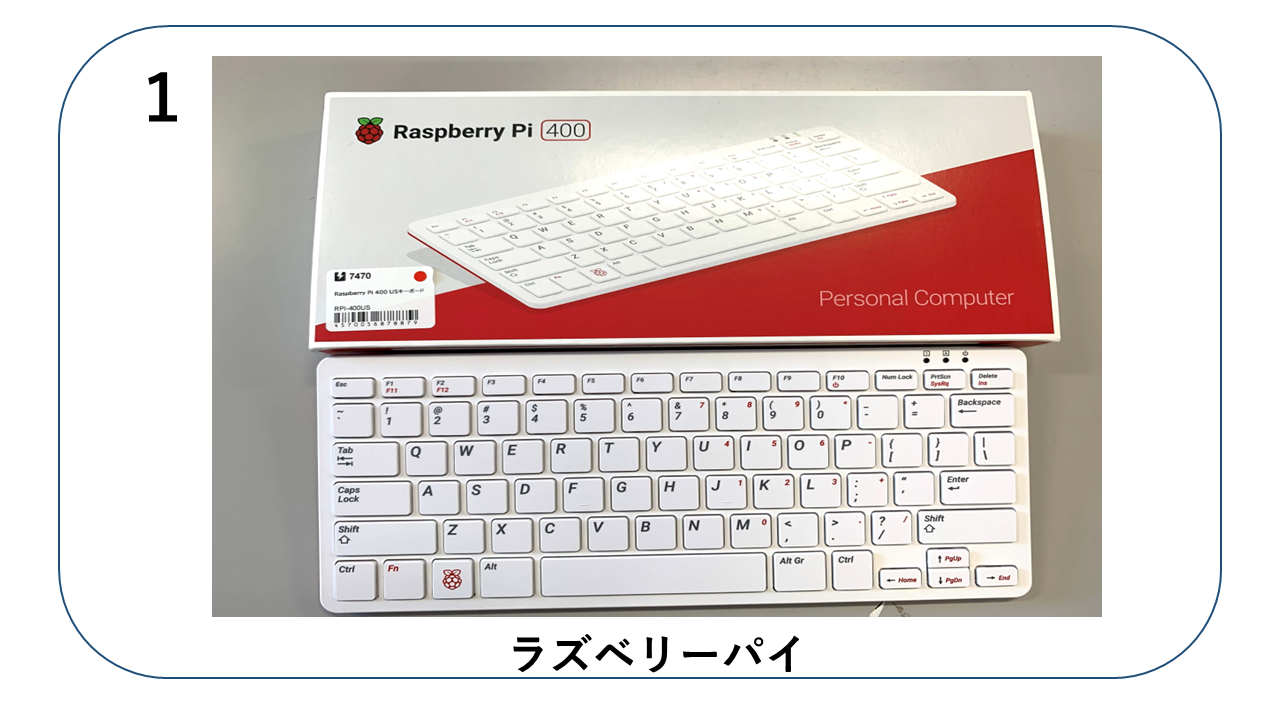
\includegraphics[width=0.22\textwidth]{textbook-img009-2023.png}
   &
		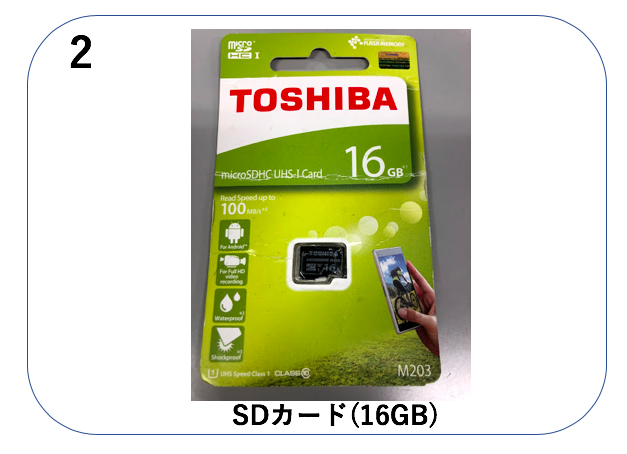
\includegraphics[width=0.22\textwidth]{textbook-img010.png} &

  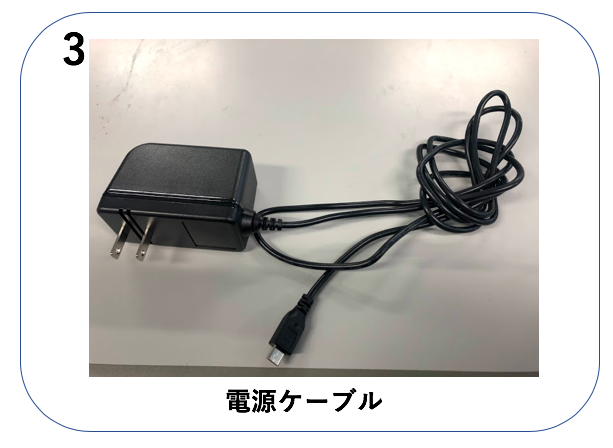
\includegraphics[width=0.22\textwidth]{textbook-img007.png}
   &
  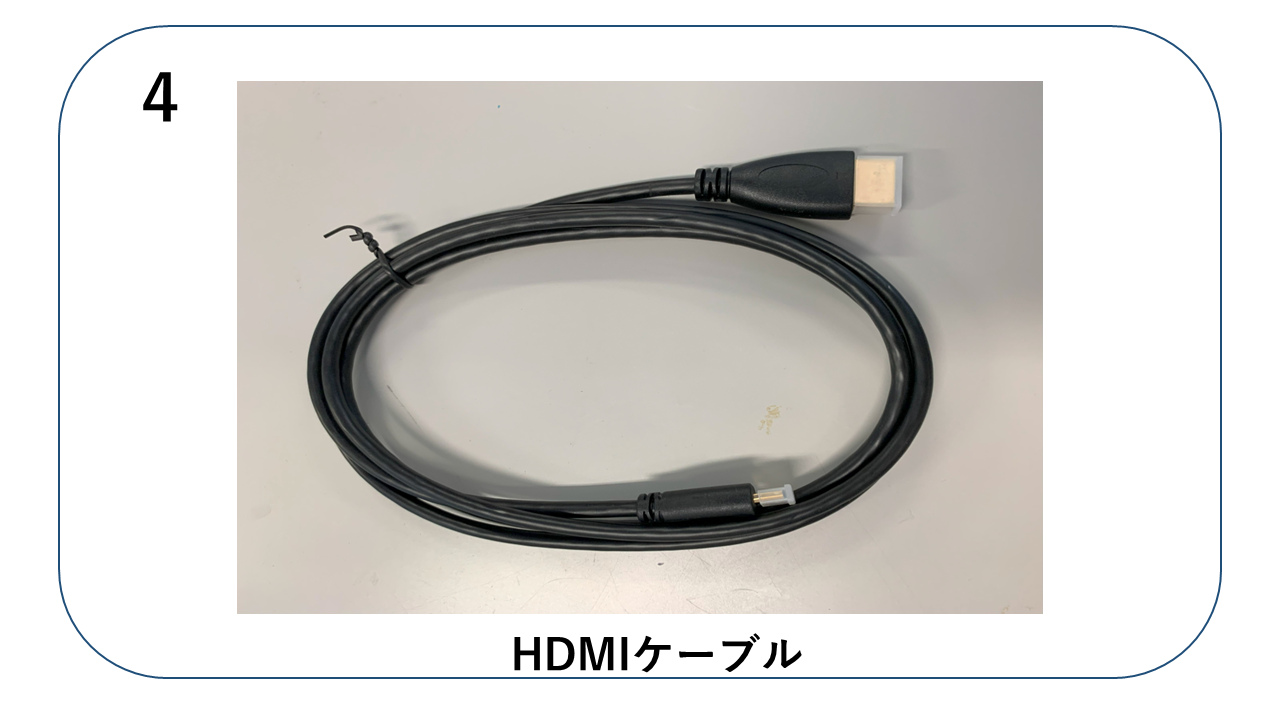
\includegraphics[width=0.22\textwidth]{textbook-img008-2023.png} \\

  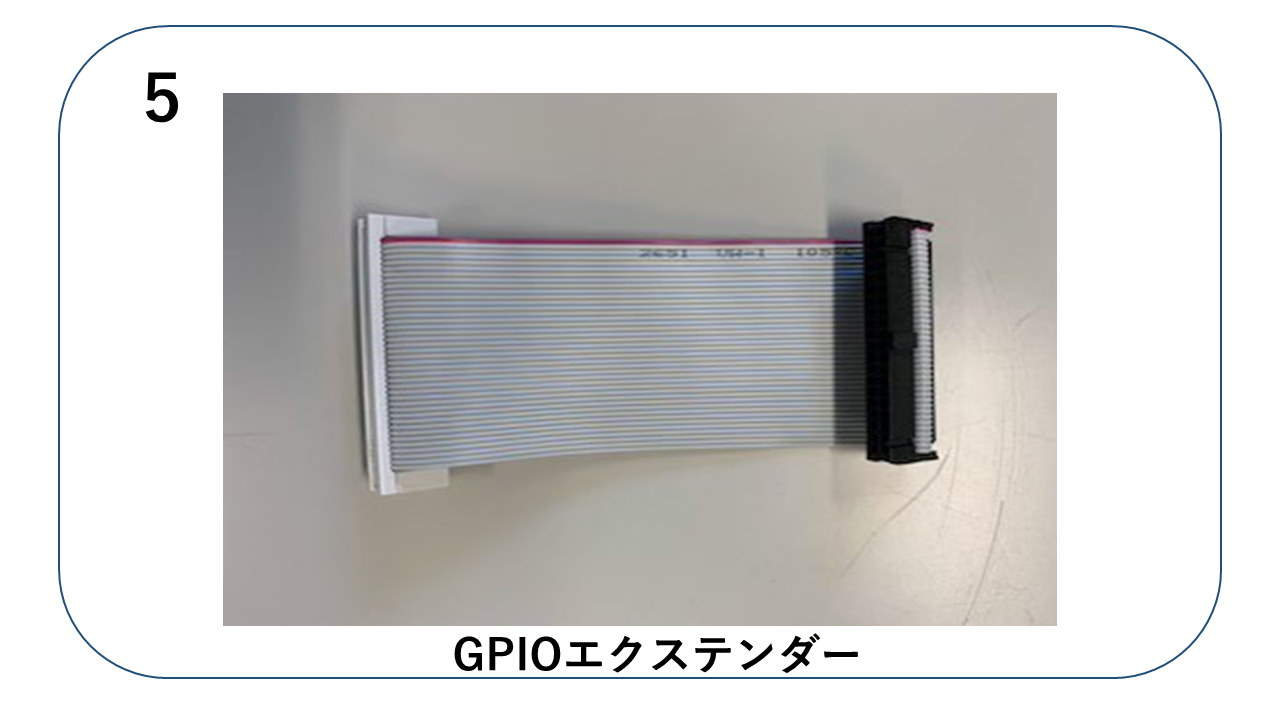
\includegraphics[width=0.22\textwidth]{textbook-img005-2023.png}
   &
		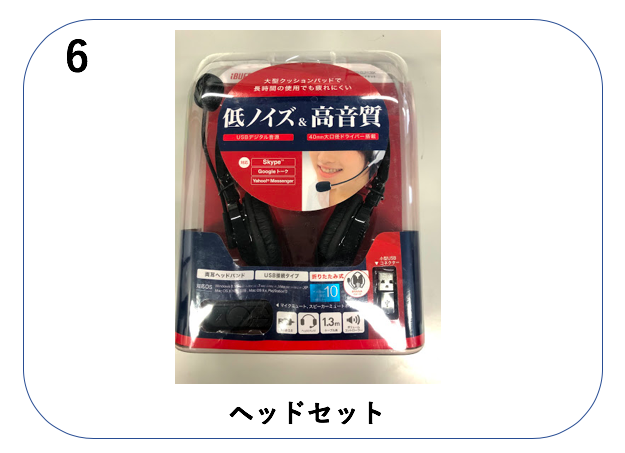
\includegraphics[width=0.22\textwidth]{textbook-img006.png} &

  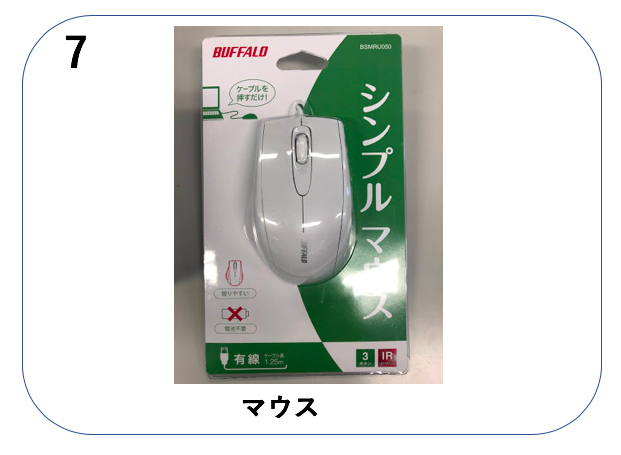
\includegraphics[width=0.22\textwidth]{textbook-img003.png}
   &
  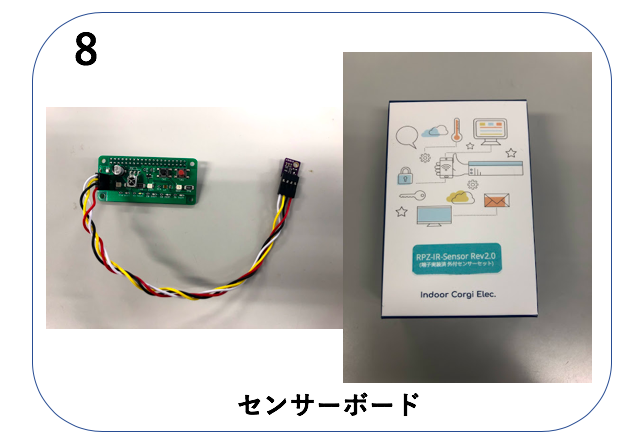
\includegraphics[width=0.22\textwidth]{textbook-img004.png} \\

  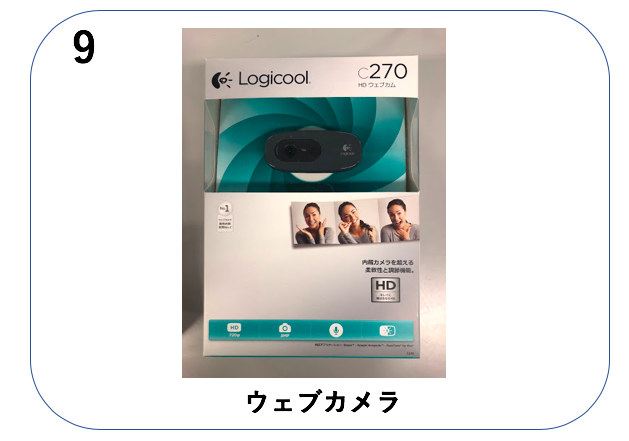
\includegraphics[width=0.22\textwidth]{textbook-img002.png}
   &
		\begin{minipage}{0.22\textwidth}
			\begin{center}
		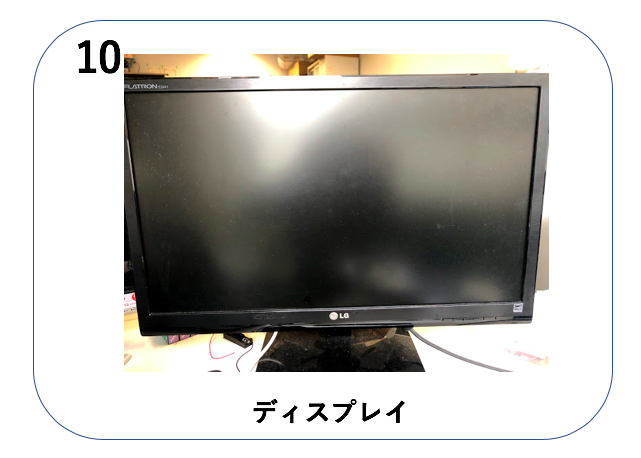
\includegraphics[width=\textwidth]{textbook-img001.png}\\
			{\color{red}貸し出し品}
			\end{center}
		\end{minipage}
			&
\end{tabular}

\end{frame}



\begin{frame}[fragile]
	\frametitle{ラズベリーパイについて:テキスト P.5~~~\raisebox{-3mm}{
\includegraphics[width=0.1\textwidth]{raspberry}}}
	イギリスで生まれた小型のコンピュータ\\
	短くラズパイとも呼ばれています。\\
			\noindent{\large\bf 特徴} ~\\
			\vfill
				\begin{itemize}
					\item キーボード一体型で、キーボードが必要ない
					\item 普通のパソコンのように使える
					\item プログラミングのべんきょうに向いている
					\item モータやライトをせいぎょできる
				\end{itemize}
\end{frame}


\begin{frame}[fragile]
	\frametitle{ラズパイを使う時の注意:テキスト P.5~~~\raisebox{-3mm}{
\includegraphics[width=0.1\textwidth]{raspberry}}}
	\begin{columns}[b]
		\begin{column}{0.8\textwidth}
				\begin{itemize}
					\item 水などぬれているものをラズベリーパイ本体につけないようにしましょう
					\item ラズベリーパイをはじめコンピュータなどは熱に弱いのですごく暑い部屋では使わないようにしましょう
					\item ラズベリーパイをらんぼうに扱うのはやめましょう
					\item 他の人に簡単には分からないユーザー名とパスワードを使おう
				\end{itemize}
				\end{column}
		\begin{column}{0.2\textwidth}
	 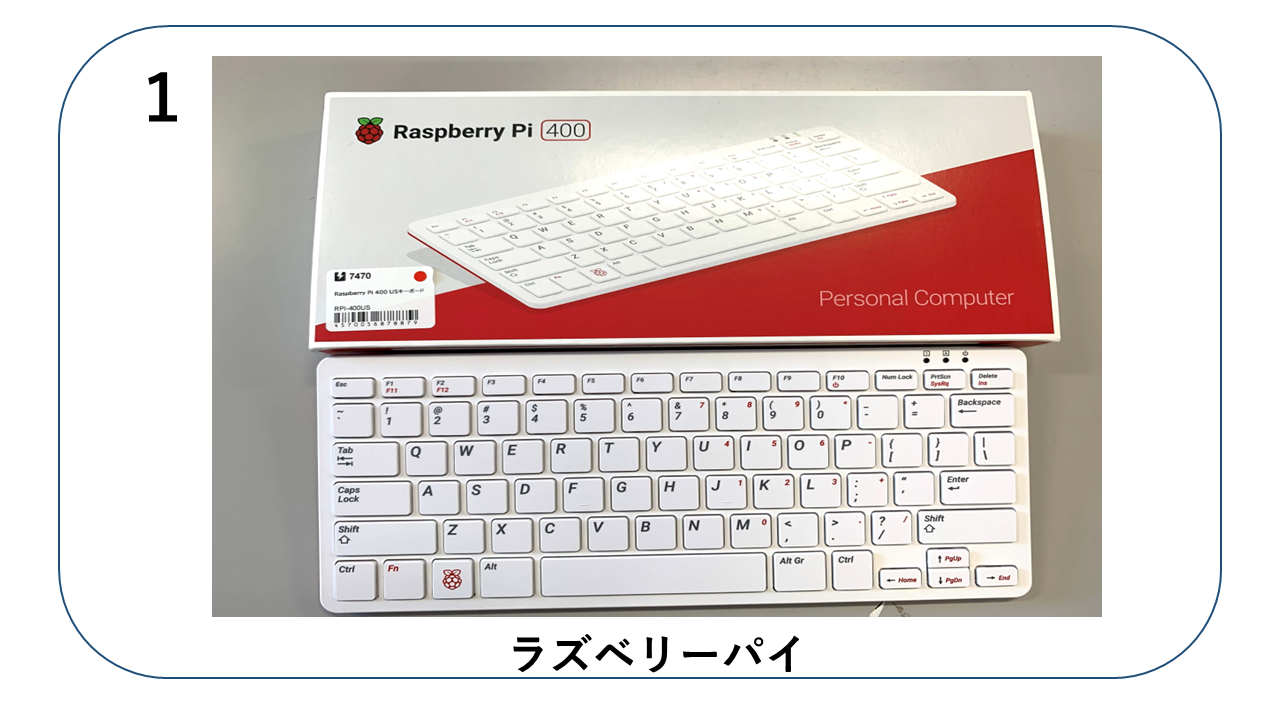
\includegraphics[width=\textwidth]{textbook-img009-2023.png}
				\end{column}
				\end{columns}

\end{frame}




\begin{frame}[fragile]
	\frametitle{ユーザー名とパスワードの注意(1):テキスト P.6?~~~\raisebox{-3mm}{
\includegraphics[width=0.1\textwidth]{raspberry}}}
	ラズパイのユーザー名とパスワードは重要な情報です。\\
	他の人に簡単に盗まれないようにしてください。\footnote{出典: 総務省『国民のための情報セキュリティサイト』\url{https://www.soumu.go.jp/main_sosiki/joho_tsusin/security_previous/kiso/k02_pass.htm}
	}
	\begin{columns}[b]
		\begin{column}{0.8\textwidth}
				\begin{itemize}
					\item 他人に自分のユーザー名とパスワードを知られてしまうと、不正にラズパイに入られることがあります。
					\item 自分のラズパイが、他のサーバーへの攻撃に使われる「踏み台」となると、持ち主が攻撃者だと疑われます
					\item ネットショップなどのシステムへ入るためのパスワードを盗まれたりします。
				\end{itemize}
				\end{column}
		\begin{column}{0.2\textwidth}
	 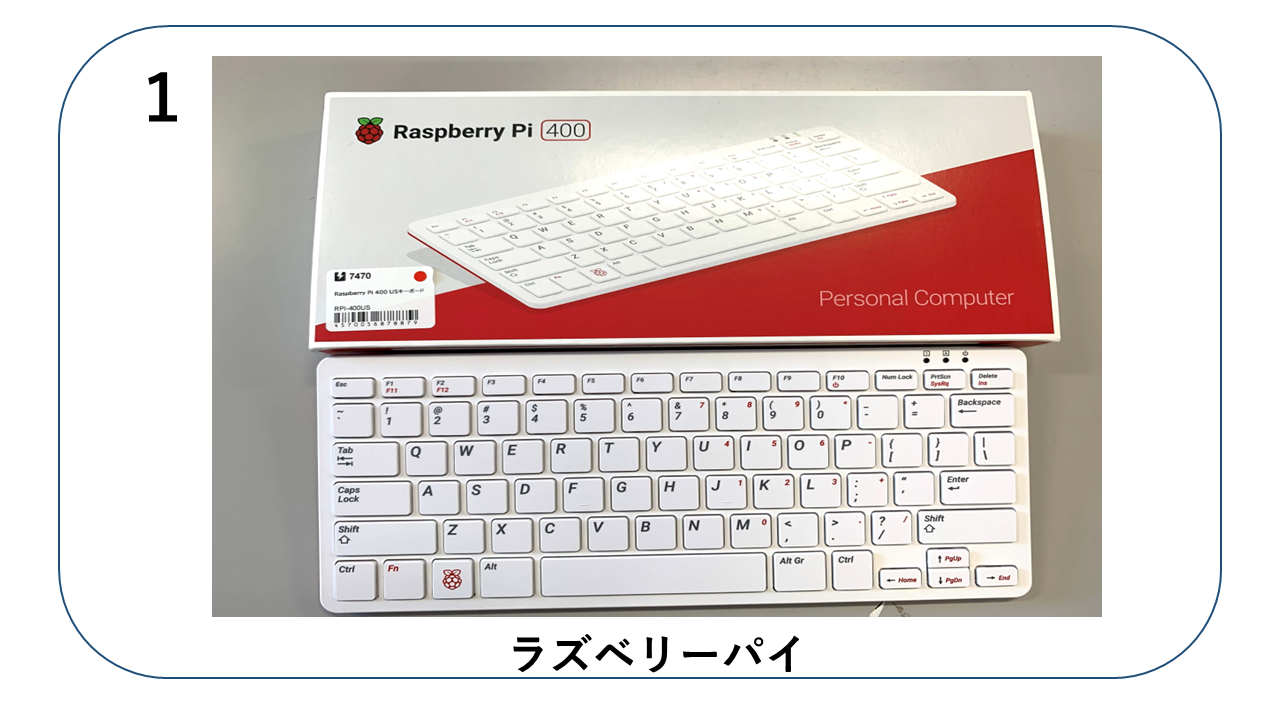
\includegraphics[width=\textwidth]{textbook-img009-2023.png}
				\end{column}
				\end{columns}

\end{frame}




\begin{frame}[fragile]
	\frametitle{ユーザー名とパスワードの注意(2):テキスト P.6?~~~\raisebox{-3mm}{
\includegraphics[width=0.1\textwidth]{raspberry}}}
	ラズパイのユーザー名とパスワード\\

	          \begin{itemize}
            \item
                  ユーザー名は小文字、数字、-、のみ使用可能。
            \item
                パスワードは8文字以上16文字以下。
            \item
                パスワードには以下の四つのカテゴリタイプの文字の内、三つのカテゴリタイプの文字を入れる必要がある。
          \end{itemize}
            \centering
            \begin{tabular}{|c|c|}
            \hline
                タイプ & 実際に使用可能な文字 \\
                \hline
                大文字& ABCDEFGHIJKLMNOPQRSTUVWXYZ\\
                \hline
                小文字& abcdefghijklmnopqrstuvwxyz\\
                \hline
                数字 &0123456789\\
                \hline
                英数字以外の文字&~!@\#\$\%\textasciicircum\&*()\_+`\{\}\textbar[]\textbackslash:";'$<>$?,./\\
                \hline
            \end{tabular}
\vfill
	\begin{center}
		\color{red}{\large 自分のユーザー名とパスワードを決め、テキストに書いておこう 問題1-1}
	\end{center}


\end{frame}

\begin{frame}[fragile]
	\frametitle{問題集:テキスト P.8 \raisebox{-3mm}{
\includegraphics[width=0.1\textwidth]{raspberry}}}
	教科書を読んで問題を解いてみよう\\
	\begin{itemize}
		\item
			問題1-2を解こう
		\item
			問題1-3を解こう
		\item
			問題1-4を解こう
	\end{itemize}
	\vfill
	\large\textbf{わからないことは、放っておかず、すぐに TA に聞きましょう}
	\vfill
	\large\textbf{問題を解き終わったらTAに確認してもらおう}

\end{frame}




\begin{frame}[fragile]
	\frametitle{ラズパイの準備:テキスト P.6?~~~\raisebox{-3mm}{
\includegraphics[width=0.1\textwidth]{raspberry}}}

	\begin{tabular}{cccc}
		\begin{minipage}{0.23\textwidth}
    {\upshape
      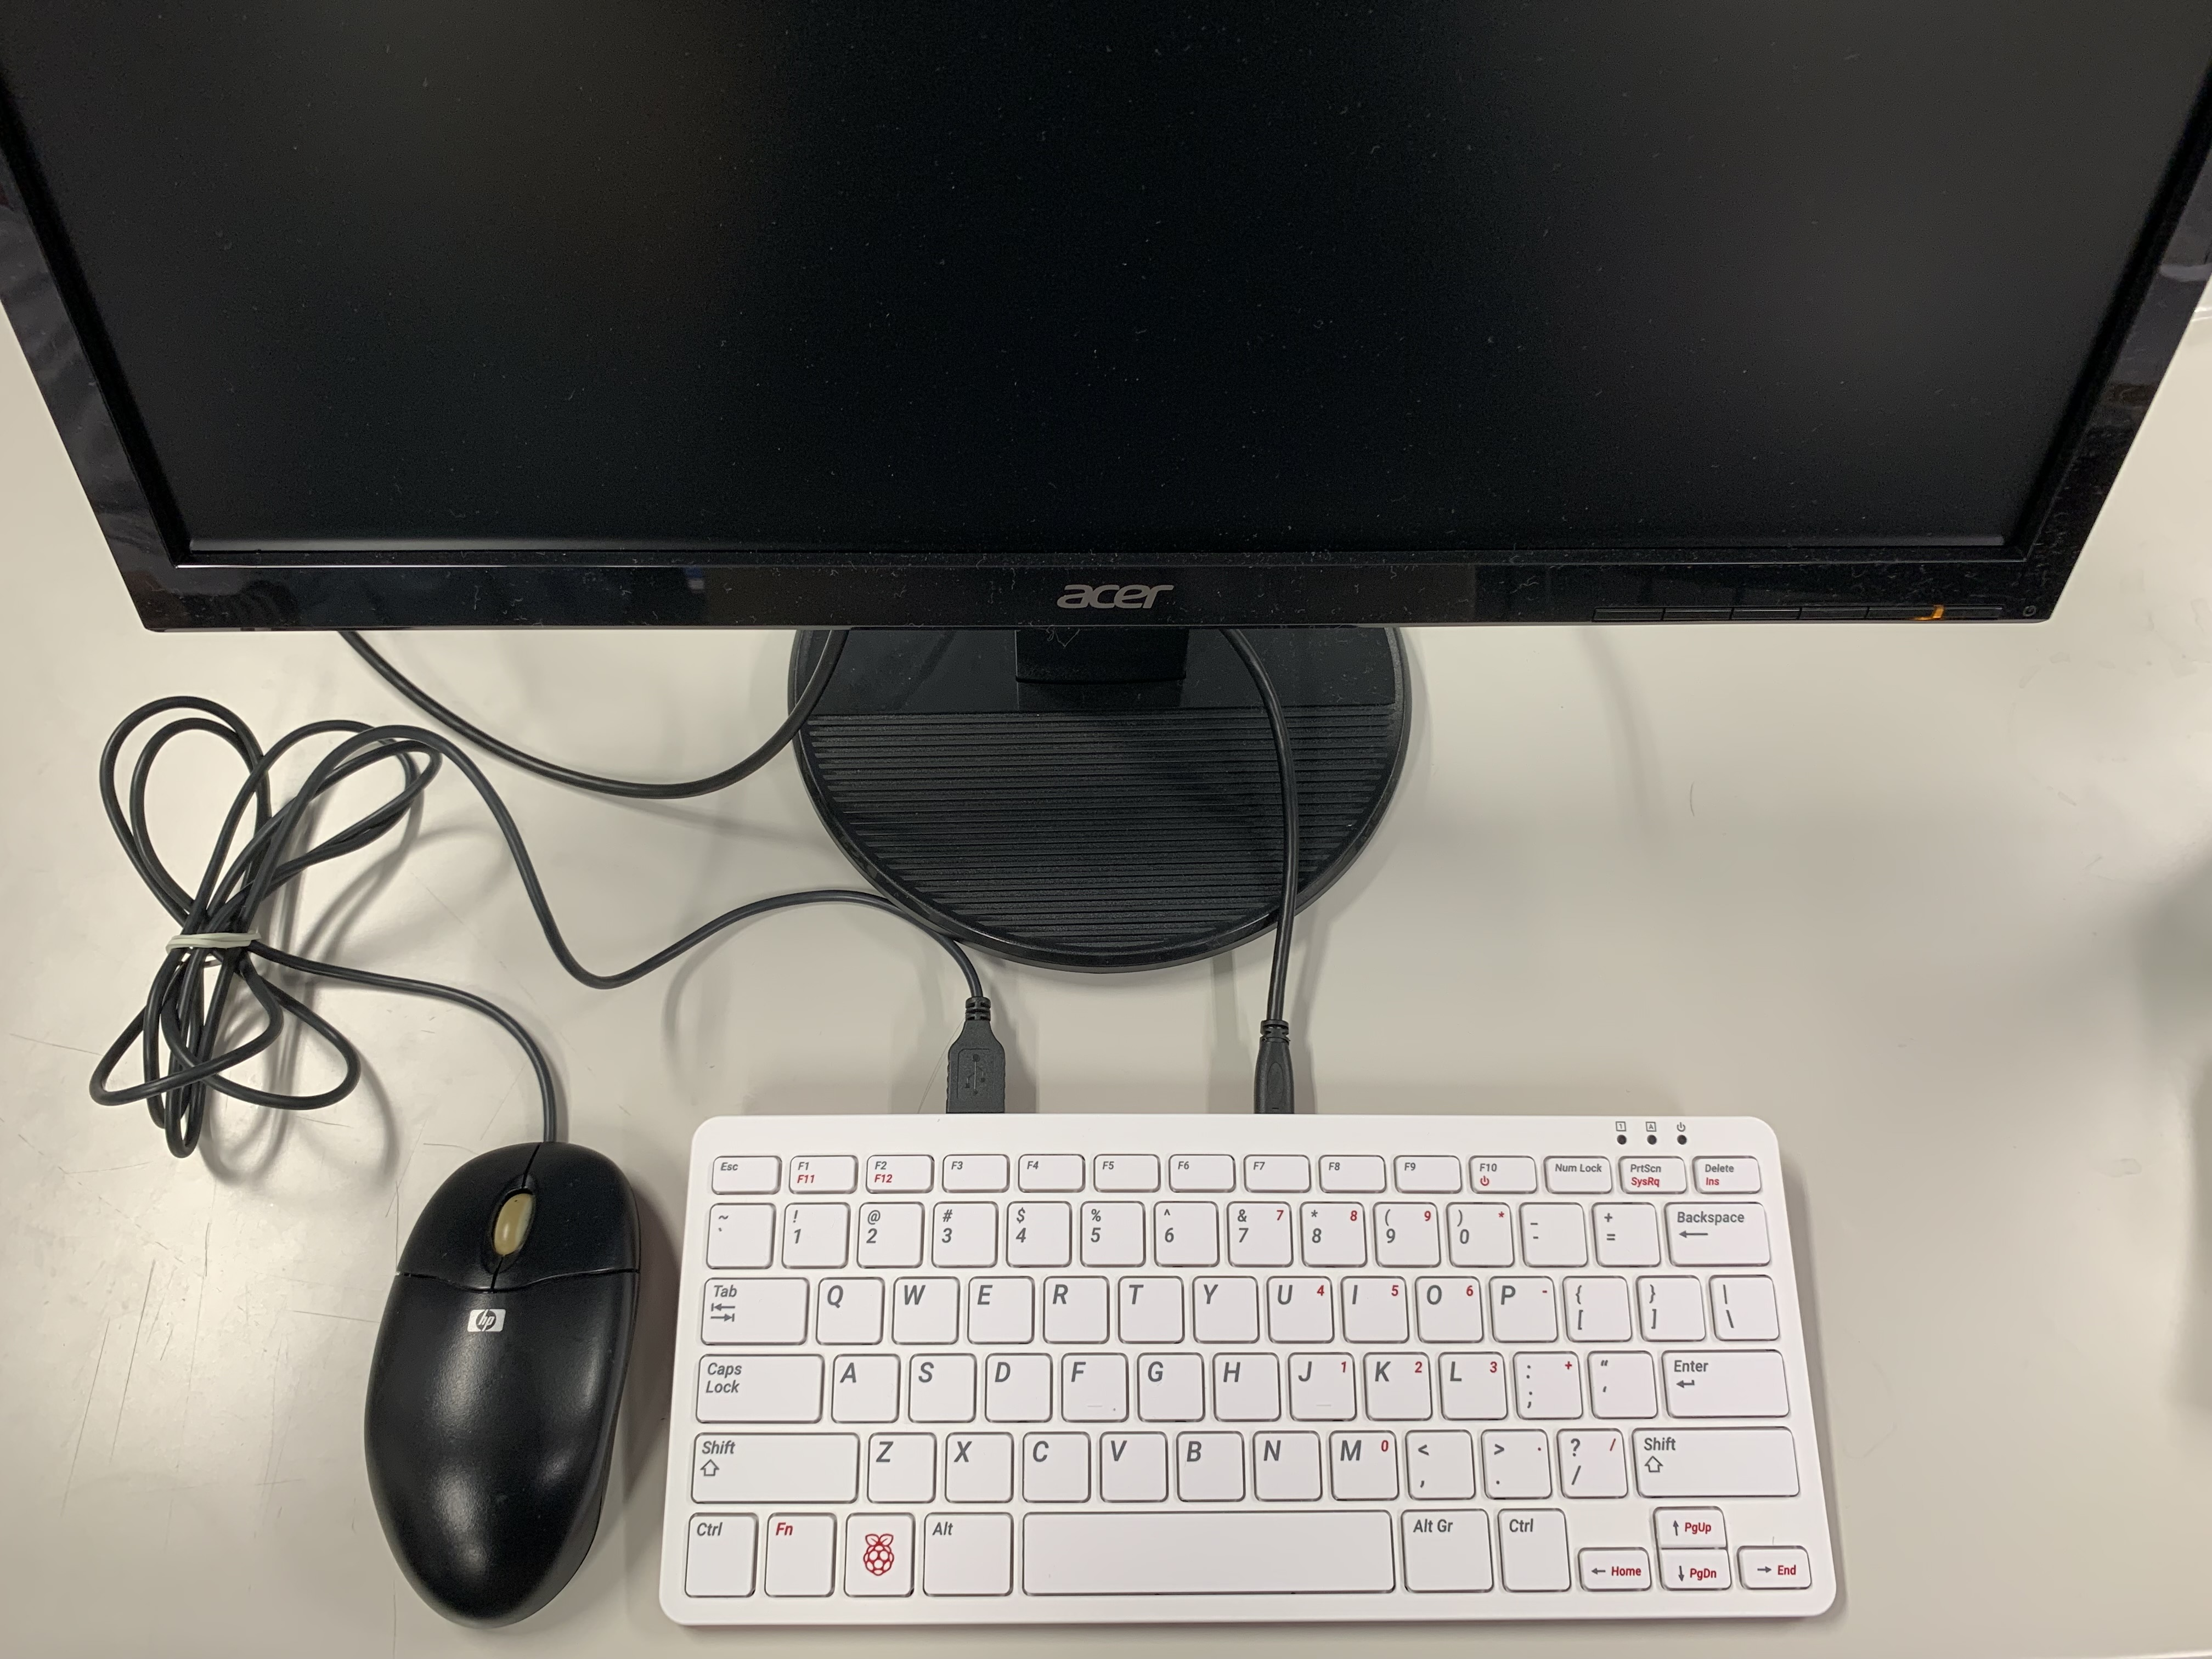
\includegraphics[width=\textwidth]{connections01-2023.jpg}
      \newline
			接続 全体図}
			\end{minipage} &
			\begin{minipage}{0.23\textwidth}
                    {\upshape
                      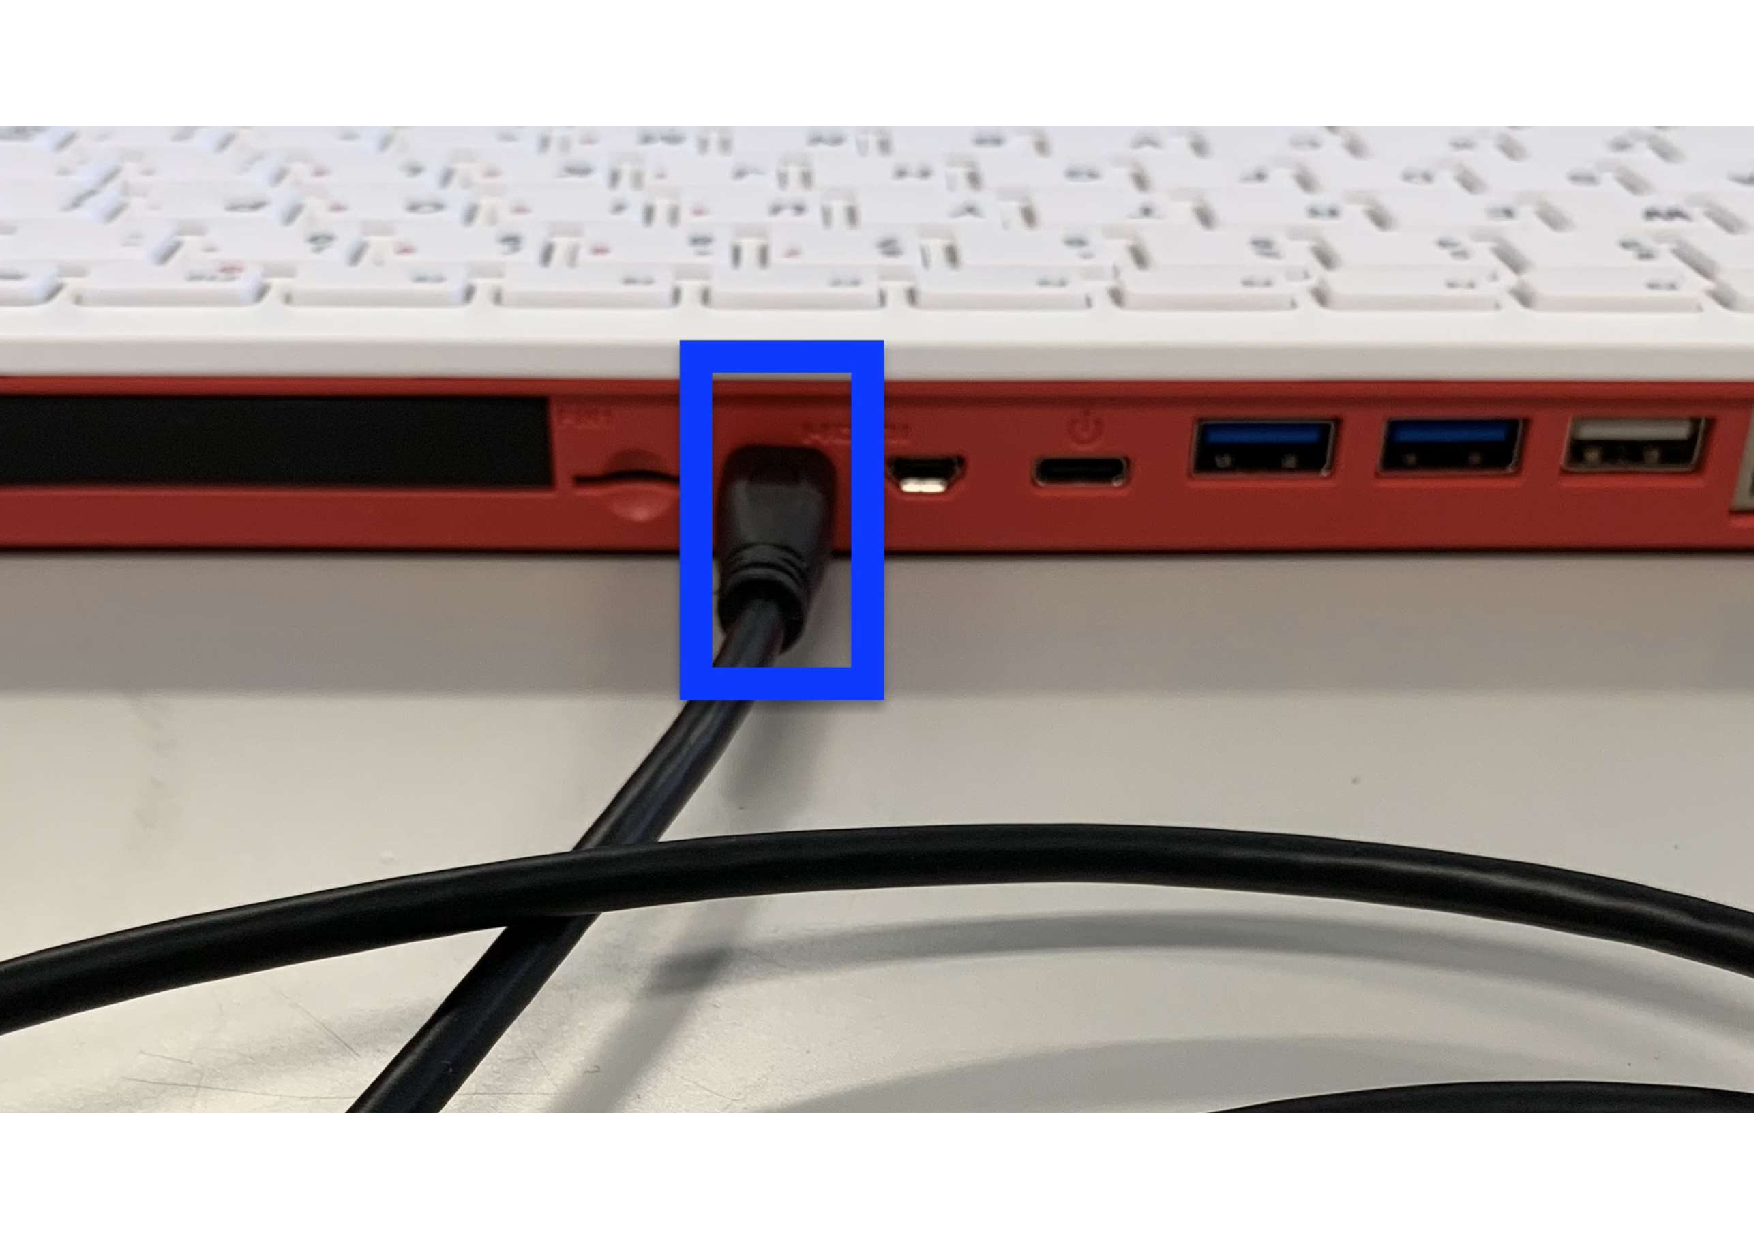
\includegraphics[width=\textwidth]{figure222023.pdf}
                      \newline
                      ラズベリーパイ HDMI}
			\end{minipage} &
			\begin{minipage}{0.23\textwidth}
                    {\upshape
                      %[Warning: Image ignored] % Unhandled or unsupported graphics:
                      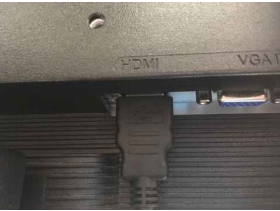
\includegraphics[width=\textwidth]{textbook-img016.png}
                      \newline
                      ディスプレイHDMI}
			\end{minipage}&
  \begin{minipage}{0.23\textwidth}
    {\upshape
      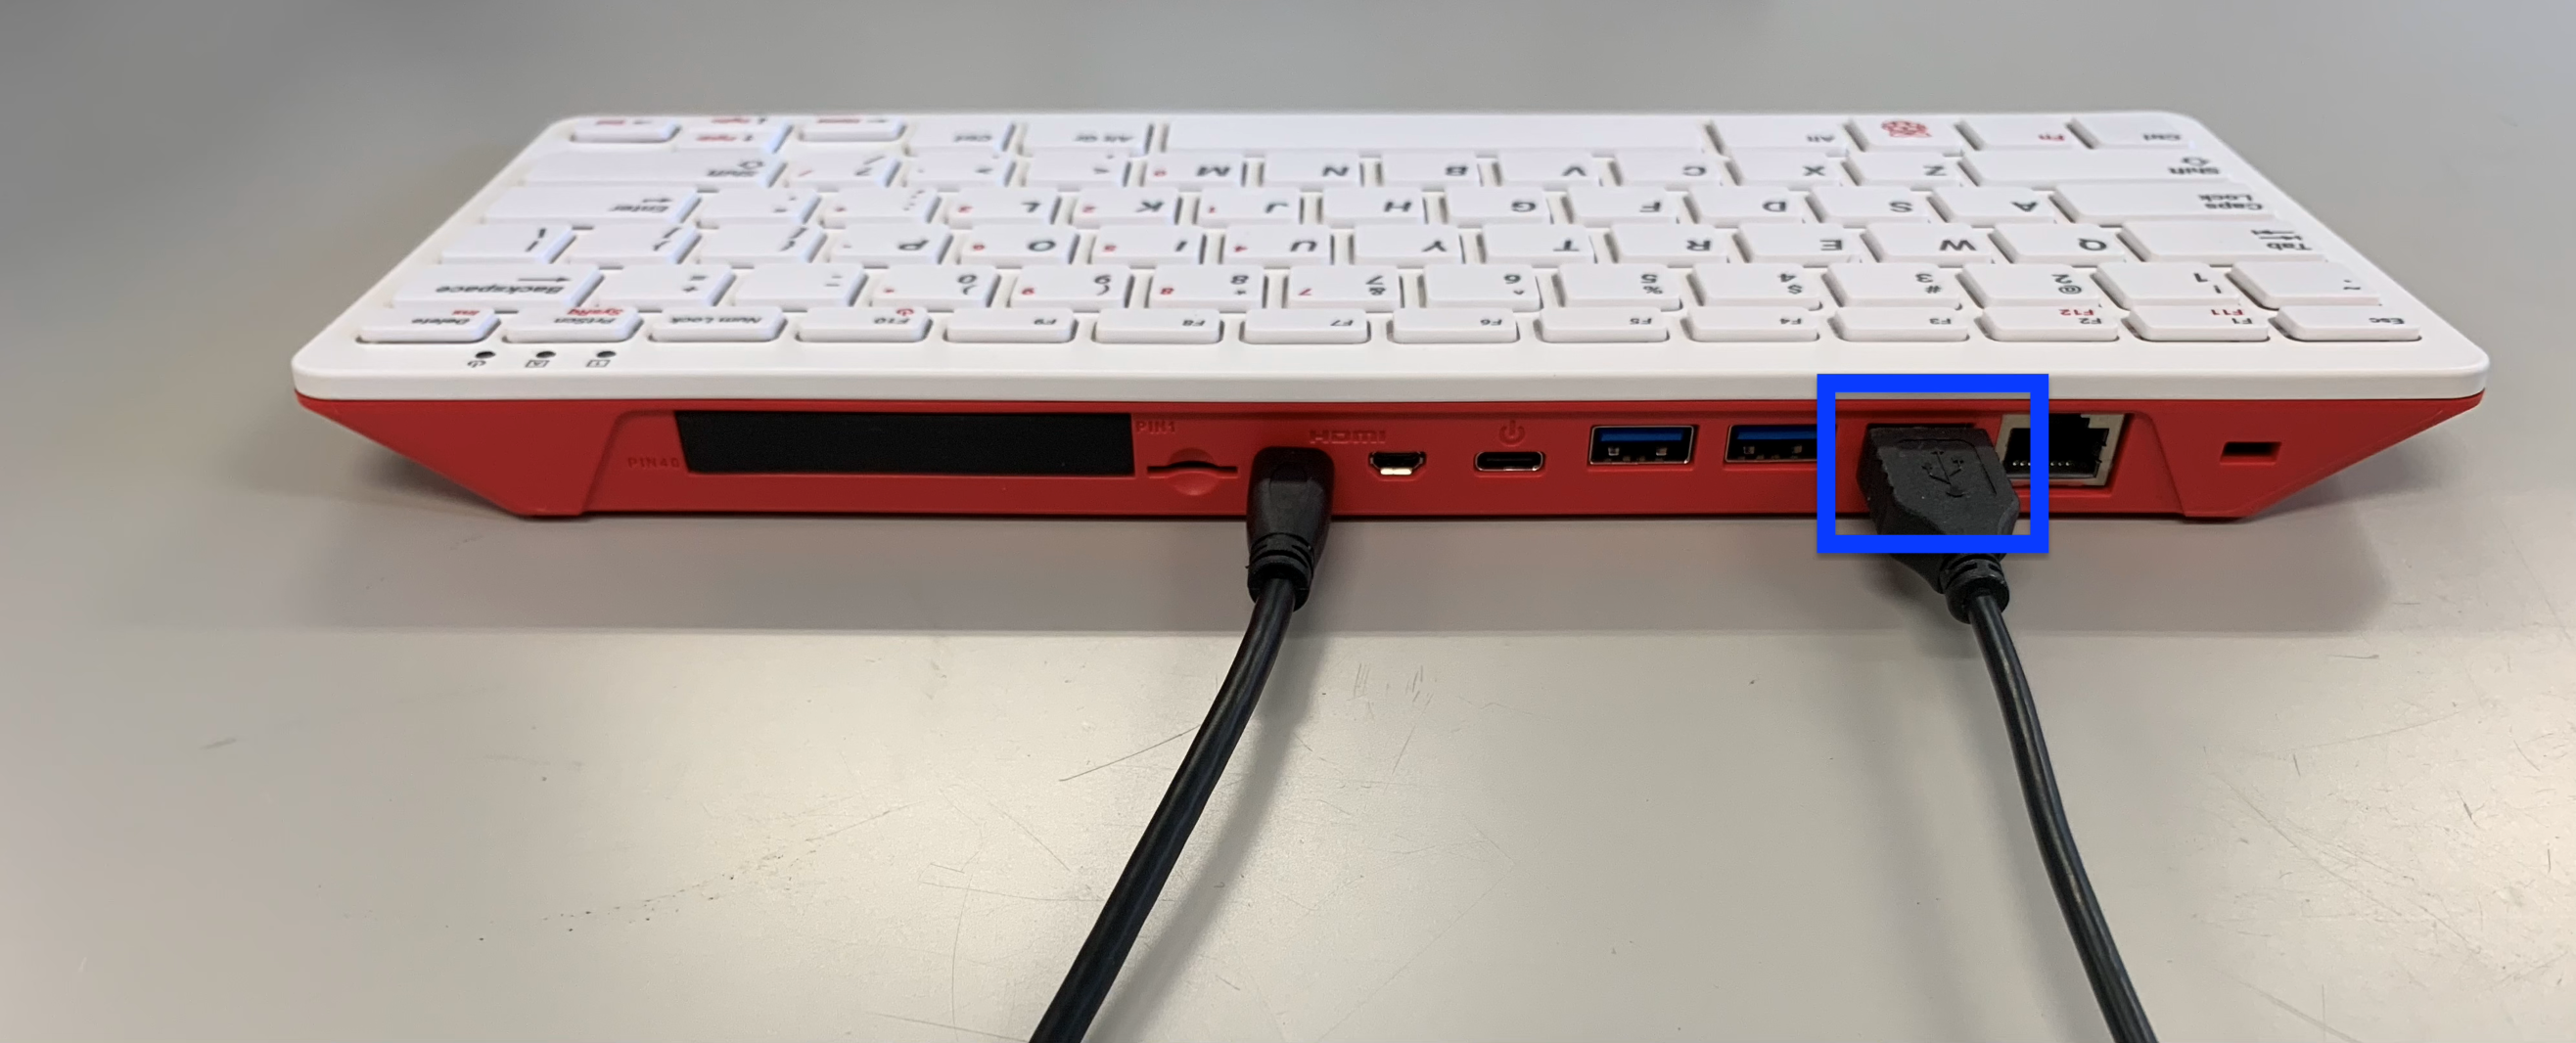
\includegraphics[width=\textwidth]{figure1.10-4.png}
      \newline
      マウス、キーボード}
  \end{minipage}\\
		 \begin{minipage}{0.23\textwidth}
                    {\upshape
                      \includegraphics[width=1\textwidth]{figure1.10-5.png}
                      \newline
                      microSDカード さしこみ}
		 \end{minipage}&
		 \begin{minipage}{0.23\textwidth}
                    {\upshape
                      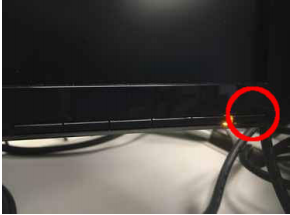
\includegraphics[width=1\textwidth]{textbook-img019.png}
                      \newline
                      モニタ でんげんボタン}
		 \end{minipage}&
		 \begin{minipage}{0.23\textwidth}
            {\upshape
              \includegraphics[width=\textwidth]{textbook-img020-2023.png}
              \newline
              ラズベリーパイ でんげん}
		 \end{minipage}&
		 \begin{minipage}{0.23\textwidth}
            {\upshape
              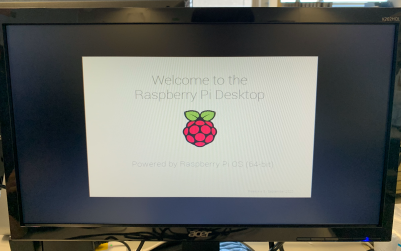
\includegraphics[width=\textwidth]{textbook-img0212023.png}
              \newline
              ラズベリーパイ 起動}
            \end{minipage} \\



	\end{tabular}


\end{frame}




\begin{frame}[fragile]
	\frametitle{ラズパイのユーザー作成:テキスト P.10-12?~~~\raisebox{-3mm}{
\includegraphics[width=0.1\textwidth]{raspberry}}}

	自分で決めたユーザー名、パスワードを使って、ラズパイにユーザーを作成しよう。
	\vfill
	\begin{tabular}{c}
		\begin{minipage}{0.32\textwidth}
                {\upshape
                  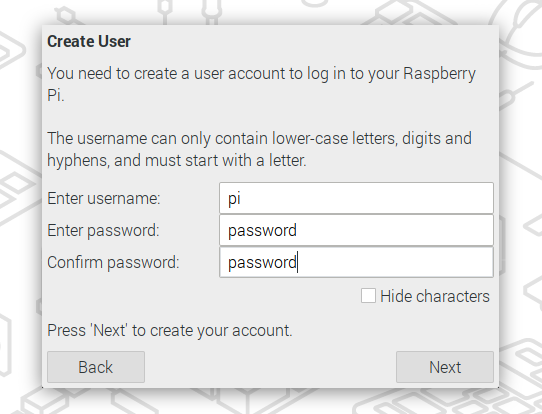
\includegraphics[width=\textwidth]{sw_image03.png}
                  \newline
                  ユーザー作成}
              \end{minipage}
	\end{tabular}


\end{frame}




\begin{frame}[fragile]
	\frametitle{ラズパイのWiFi設定:テキスト P.13?~~~\raisebox{-3mm}{
\includegraphics[width=0.1\textwidth]{raspberry}}}

	自分の班に割り当てられたWiFiネットワーク名、パスワードを使って、ラズパイをWiFiに接続しよう
	\vfill
	\begin{center}
	\begin{tabular}{cc}
		\begin{minipage}{0.32\textwidth}
                {\upshape
                  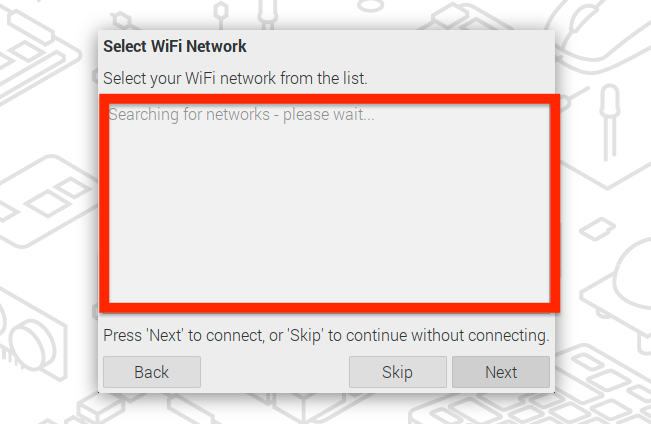
\includegraphics[width=\textwidth]{sw_image06kai.png}
                  \newline
                  Wi-Fi設定}
		\end{minipage}&
		\begin{minipage}{0.32\textwidth}
                          {\upshape
                            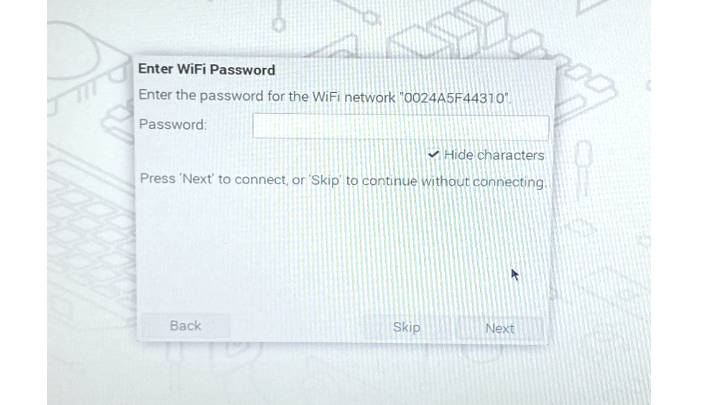
\includegraphics[width=\textwidth]{pswd_image_0404.png}
                            \newline
                            パスワード入力}
                        \end{minipage}

	\end{tabular}
	\end{center}


\end{frame}


\begin{frame}[fragile]
	\frametitle{例題1-4 アップデートをスキップしてraspberry piを始めよう P.15~~~\raisebox{-3mm}{
\includegraphics[width=0.1\textwidth]{raspberry}}}
  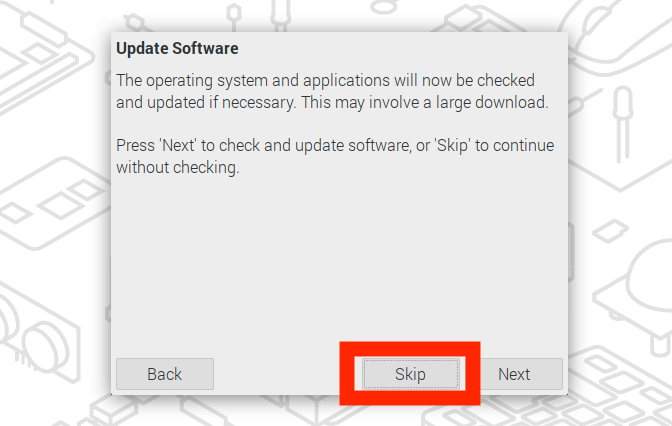
\includegraphics[width=0.47\textwidth]{sw_image07.png}
  \hfill
  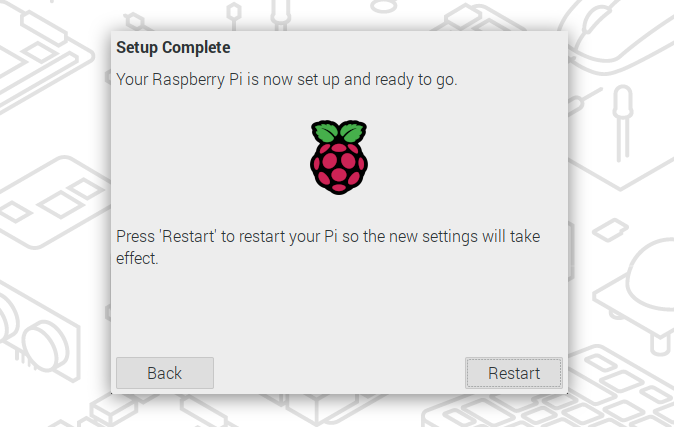
\includegraphics[width=0.47\textwidth]{sw_image08.png}
  \vfill
  \large\textbf{今回はアップデートをしないでください}
  \begin{itemize}
    \item 再起動してraspberry piを始めよう
  \end{itemize}

\end{frame}

\begin{frame}[fragile]
	\frametitle{\raisebox{-3mm}{
\includegraphics[width=0.1\textwidth]{raspberry}}休憩~~~\raisebox{-3mm}{
\includegraphics[width=0.1\textwidth]{raspberry}}}

	\huge
      \begin{itemize}
           \item 水分補給をしましょう
           \item 遠くのものを見て目を休めましょう
     \end{itemize}



\end{frame}




\end{document}
